% title page
\begin{frame}[fragile]
   \begin{center}
    \huge{子どもIT未来塾}\\

    \vspace{48pt}
	   \Large{第5回}\\
	   {\huge\bf ラズベリーパイの使い方・\\
	   \huge\bf 自己紹介ページを作ろう}\\
    \vspace{24pt}
    \large{奥山祐市先生}\\
    \vspace{10pt}
    \large{\the\year 年 8月19日}
  \end{center}
\end{frame}

\begin{frame}
    \frametitle{教材の更新の方法 1/2}
    \begin{center}
        \begin{figure}
            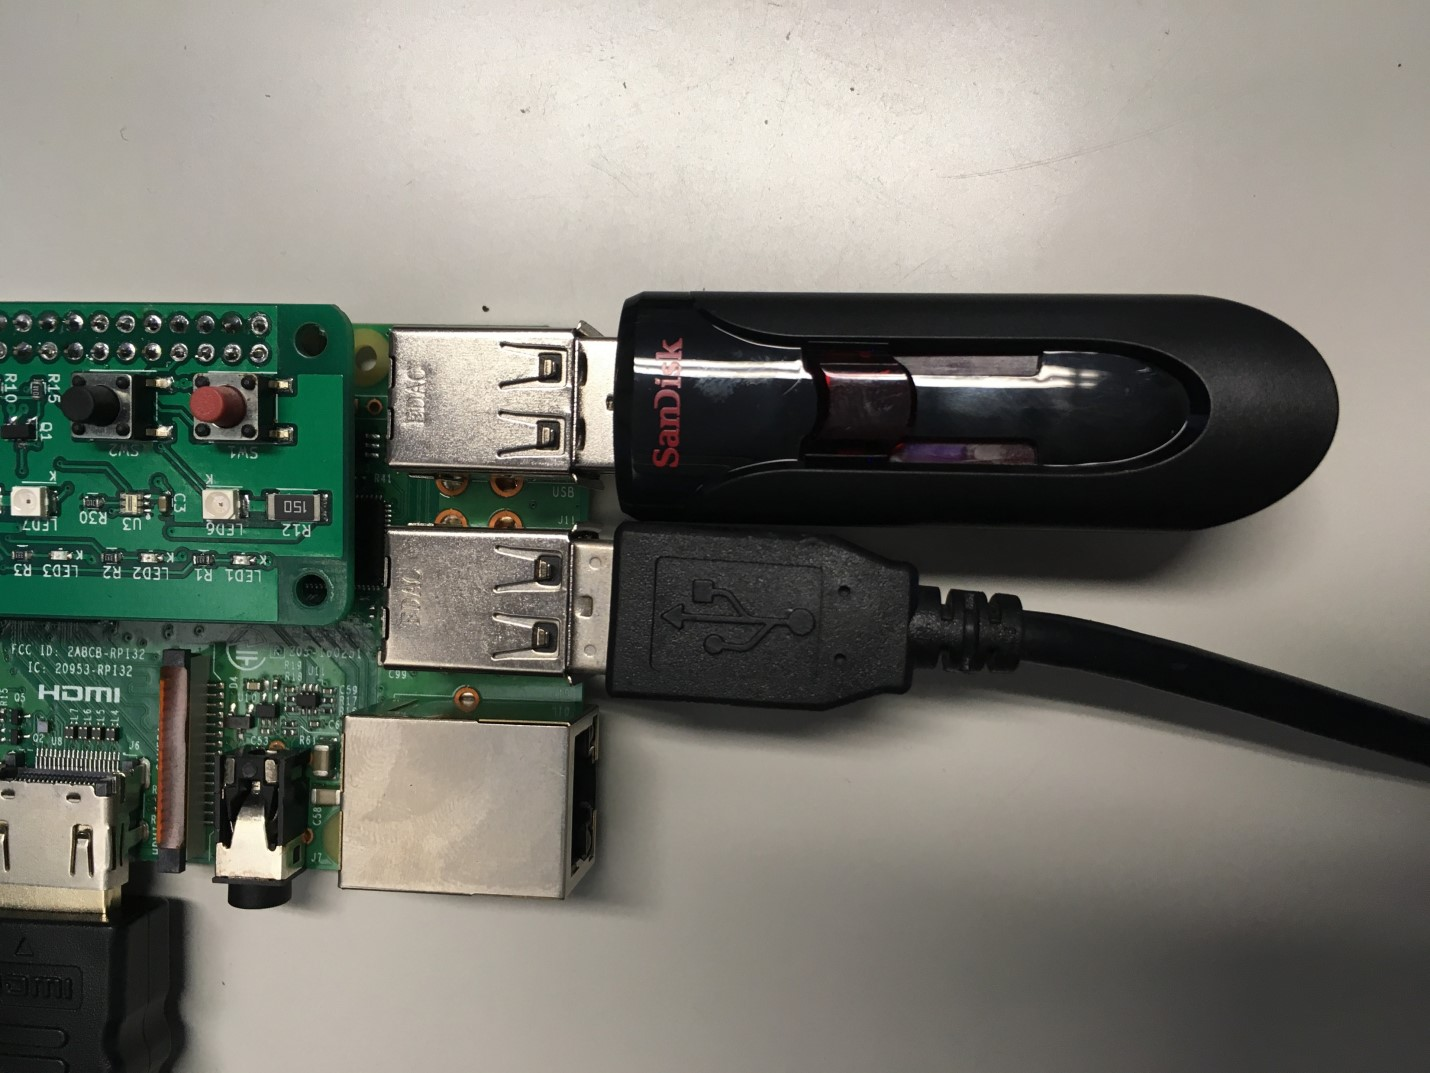
\includegraphics[width=0.8\textwidth]{images/slide/how_to_install_usb.png}
        \end{figure}
    \end{center}
\end{frame}

\begin{frame}[fragile]
    \frametitle{教材の更新の方法 2/2}
    \begin{center}
        \begin{figure}
            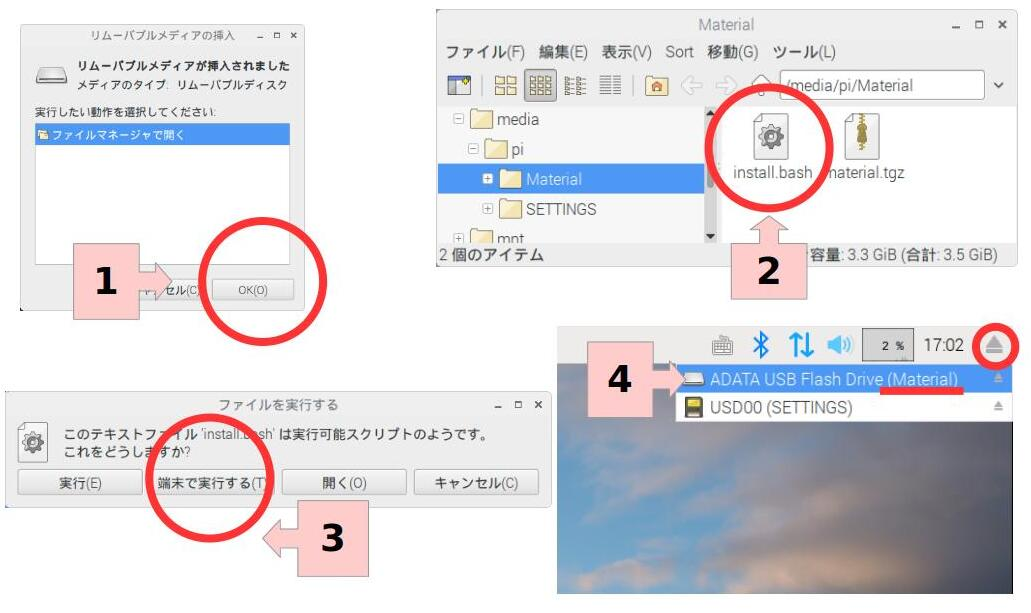
\includegraphics[width=\textwidth]{images/slide/how_to_update.jpg}
        \end{figure}
    \end{center}
\end{frame}

\begin{frame}[fragile]
    \frametitle{目次}
    \begin{enumerate}
        \item センサーについて知ろう
        \item FaBoのセンサーを使ってみよう
        \item 赤外線について知ろう
        \item 赤外線を送信・受信してみよう
        \item 赤外線を使って家電を動かしてみよう
        \item 演習
    \end{enumerate}
\end{frame}
